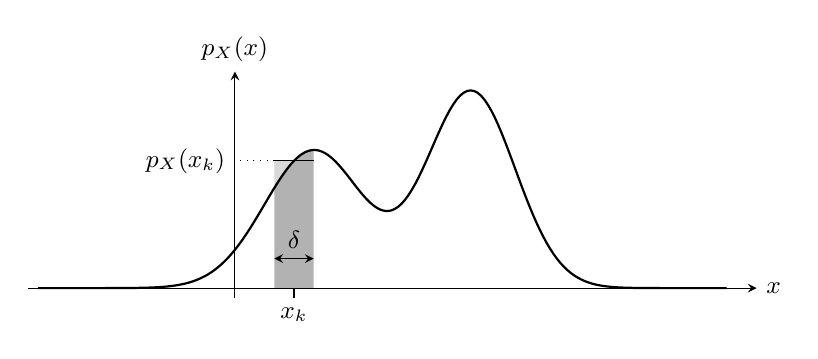
\begin{tikzpicture}
\shorthandoff{>}
%
% Cuantificacion de X
\begin{scope}[xscale=2.5,yscale=2.5]
%
\pgfmathsetmacro{\c}{.4};
\pgfmathsetmacro{\d}{1.2};
\pgfmathsetmacro{\s}{8};
\pgfmathsetmacro{\t}{10};
\pgfmathsetmacro{\a}{.7};
\pgfmathsetmacro{\b}{1};
%
\pgfmathsetmacro{\xk}{.3};
\pgfmathsetmacro{\dx}{.2};
%
\draw[>=stealth,->] (-1.05,0)--(2.65,0) node[right]{\small $x$};
\draw[>=stealth,->] (0,-.05)--(0,1.1) node[above]{\small $p_X(x)$};
%
% lei de proba
\draw[thick,domain=-1:2.5,samples=200] plot (\x,{(\a*exp(-\s*(\x-\c)^2)+\b*exp(-\t*(\x-\d)^2))});
%
% dominio alrededor de xk
\fill[domain=\xk-\dx/2:\xk+\dx/2,samples=20,opacity=.3]
({\xk-\dx/2},0)--
plot (\x,{(\a*exp(-\s*(\x-\c)^2)+\b*exp(-\t*(\x-\d)^2))})--
({\xk+\dx/2},0);
%
% xk y delta
\draw (\xk,0)--(\xk,-.05) node[below]{\small $x_k$};
\draw[>=stealth,<->] ({\xk-\dx/2},.15)--({\xk+\dx/2},.15);
\draw (\xk,.15) node[above]{\small $\delta$};
%
% recta sobre delta a altura de p(xk)
\draw ({\xk+\dx/2},{(\a*exp(-\s*(\xk-\c)^2)+\b*exp(-\t*(\xk-\d)^2))})--
({\xk-\dx/2},{(\a*exp(-\s*(\xk-\c)^2)+\b*exp(-\t*(\xk-\d)^2))});
\draw[dotted] ({\xk-\dx/2},{(\a*exp(-\s*(\xk-\c)^2)+\b*exp(-\t*(\xk-\d)^2))})--
(0,{(\a*exp(-\s*(\xk-\c)^2)+\b*exp(-\t*(\xk-\d)^2))}) node[left]{\small $p_X(x_k)$};
%
% dominio equivalente alrededo de xk
\fill[domain=\xk-\dx/2:\xk,samples=20,opacity=.15]
plot (\x,{(\a*exp(-\s*(\x-\c)^2)+\b*exp(-\t*(\x-\d)^2))})--
({\xk-\dx/2},{(\a*exp(-\s*(\xk-\c)^2)+\b*exp(-\t*(\xk-\d)^2))});
\end{scope}
\end{tikzpicture}